\chapter{Lattice Quantum Chromodynamics}
\label{chap:latticeqcd}

As mentioned in Sec. \ref{sec:qcd}, at low energies QCD becomes non-perturbative. In other words, the coupling $\alpha_s$ becomes $\mathcal{O}(1)$, and an expansion in $\alpha_s$ (as in perturbation theory) will not be dominated by the leading orders. In order to calculate observables of low energy QCD (like hadronic form factors), we require an alternative to perturbation theory.

The expectation value of an observable $\mathcal{O}$ in QCD can be expressed as a path integral:
\begin{align}
  \langle \mathcal{O} \rangle = {1\over Z}\int [dG d\psi d\bar{\psi}] \, \mathcal{O} \, e^{iS[G,\psi,\bar{\psi}]},
\end{align}
where $G$ is the gauge field, $\psi$($\bar{\psi}$) are the (anti)fermion fields, $S$ is the classical action, and $[dG d\psi d\bar{\psi}]$ denotes integration over all configurations of the gauge and fermion fields. $Z$ is the partition function. In the perturbative approach, we would expand $\exp(-\text{interacting part of }S )$ resulting in a power series in the gauge coupling populated by Feynman diagrams.

We must instead carry out the integral directly, by numerical brute force. Since it is not numerically feasible to carry out an infinite number of integrals, one must approximate spacetime as a discrete 4-dimensional lattice with spacing $a$ between lattice sites, finite spacial volume $L_x^3=(aN_x)^3$ and finite temporal extent $L_t=aN_t$ ($N_{x,t}\in \mathbb{N}$). The functional integral can be replaced with
\begin{align}
  \int [dG d\psi d\bar{\psi}] = \prod_{n} \int dU(x_n) d\psi(x_n) d\bar{\psi}(x_n),
\end{align}
where $n$ is a 4-vector with integer components labelling the sites, and $x_n^{\mu} = an^{\mu}$.
This has a second benefit which is to naturally regularize the theory with a momentum cutoff $\Lambda \sim \pi/a$. The gauge field has been replaced with the {\it{gauge link}} $U$, to be defined in the following section.

Typically one uses lattices that have periodic boundary conditions in the temporal direction, i.e $\psi(x+aN_t \hat{t}) = \psi(x)$. This reduces unwanted effects in expectation values of operators due to the finite temporal extend. In all the work in this thesis we use periodic temporal boundary conditions.

To avoid having to integrate over imaginary numbers (equivalently to avoid the scourge of the {\it{sign problem}} \cite{deForcrand:2010ys}), one also performs a {\it{Wick rotation}}. This is the redefinition $t\to it$, which changes the metric from Minkowski to Euclidean, and changes the weight $\exp(iS) \to \exp(-S)$. This has the advantage that it turns the quantum path integral into simply an average in statistical mechanics, this means we can apply all of the machinery of statistical mechanics to computing expectation values.

To obtain the 'real world' result for some expectation value, where real world means $a=0$, one must perform the path integral at a number of different $a$ values, and then extrapolate the results to $a=0$.

One must choose a discretized version of the QCD action, one that becomes continuum QCD in the $a\to 0$ limit. This is a far from trivial step. There is an infinite number of choices of lattice actions that become QCD in the continuum limit. There therefore is a huge literature of different choices of discrete lattice actions.

The rest of this chapter is dedicated to motivating and detailing the choices of discretisation used in the work of this thesis.

\section{Lattice Gauge Fields}
\label{sec:gaugefields}

%Often the best way to introduce some sophisticated method or technique is to first show how the naive approach breaks down.
Imagine attempting a naive discretisation of the QCD action. Derivatives can be replaced with something like
\begin{align}
  \partial_{\mu}f(x) \to {1\over 2a} \left( f(x+a\hat{\mu}) - f(x-a\hat{\mu}) \right)
\end{align}
where $\hat{\mu}$ is the unit vector in the $\mu$ direction. The quark kinetic part of the QCD action, $\bar{q}\slashed{D}q$, becomes
\begin{align}
  {1\over 2a} \bar{q}(x)\gamma^{\mu}q(x+a\hat{\mu}) - {1\over 2a} \bar{q}(x)\gamma^{\mu}q(x-a\hat{\mu}) - ig\bar{q}(x)G_{\mu}(x)\gamma^{\mu} q(x).
\end{align}
This is no longer invariant under gauge trasforms \eqref{eq:quark_gauge_trans}, for example the first term becomes $\bar{q}(x)\Lambda(x)^{\dagger} \Lambda(x+a\hat{\mu}) q(x+a\hat{\mu})$. The finite distance between lattice sites force us to think more carefully about the interpretation of gauge symmetry on a lattice.

Formally speaking, a gauge field is a connection on a fibre bundle. I'll unpack what this means. At each point $x$, there is a space of possible color vectors that a quark field $q(x)$ could be, call it $V_x$. $V_x$ is a {\it{fibre}}. Spacetime is called the {\it{base space}} in this context, there is a fibre at each point in the base space.

The problem with our non-gauge-invariant terms above is that we are trying to compare color vectors in different fibres. To compare color vectors at two different fibres, one must {\it{parallel transport}} the vector from one point to another, according to some rule of how it should change. This rule is called the {\it{connection}}. In our case the parallel transport is a Wilson line:
\begin{align}
  \nonumber  &W(x,y) : V_y \to V_x, \\ &W(x,y) = Pe^{ig\int dc\,\cdot\, G }.
\end{align}
where $c$ is some curve between $x$ and $y$, and $P$ orders the operation of the gauge field $G$ on the fibres, i.e. it operates at $x$ first and $y$ last. A wilson line transforms under the gauge group like $W(x,y)\to \Lambda(x)W(x,y)\Lambda^{\dagger}(y)$, so operators like $\bar{q}(x)W(x,y)q(y)$ are gauge-invariant, reflecting the fact that the color vector $q(y)$ has been parallel transported into the same fibre as $\bar{q}(x)$.

\begin{figure}[htb!]
  \begin{center}
    \vspace{-10pt}
    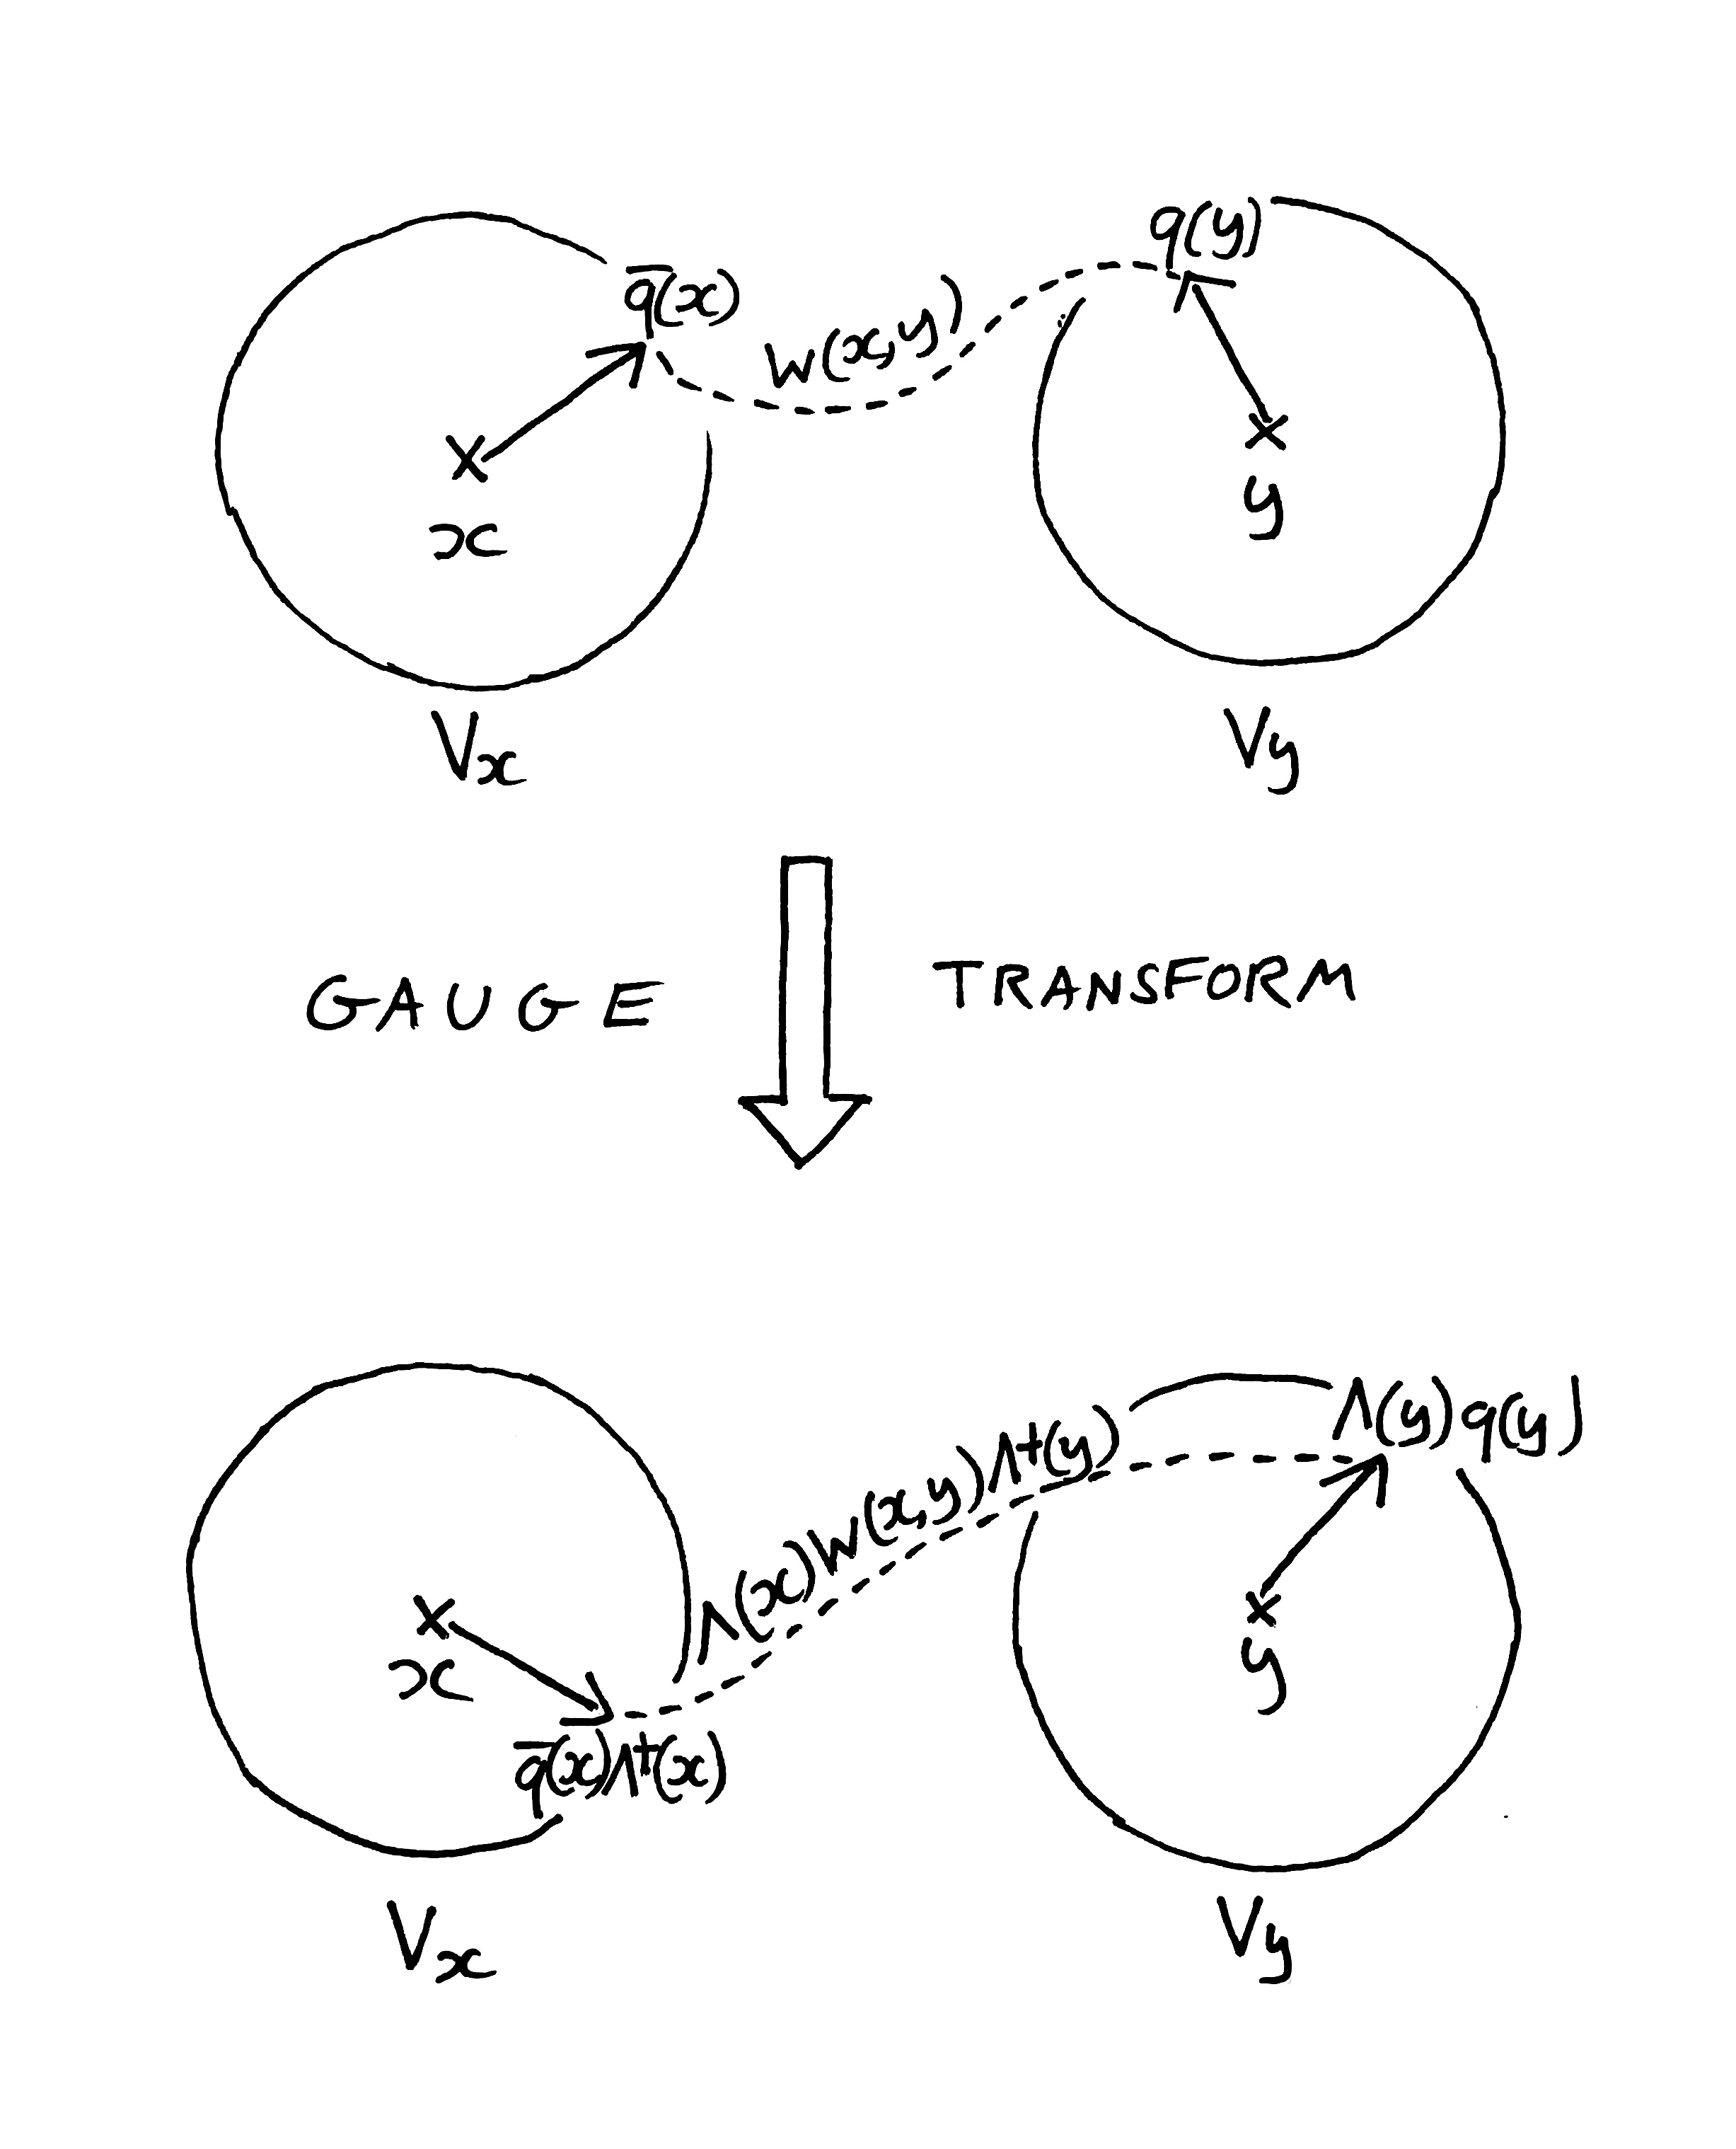
\includegraphics[width=0.55\textwidth]{images/fibres.jpg}
    \caption{Depiction of color spaces (fibres) at two points in spactime (base space) with the value of the quark field $q$ represented at each point as a color vector, and the connection $W(x,y)$ needed to compare the two color vectors. A gauge transform changes the two vectors in different ways, for the comparison to be gauge independent, the connection must also transform appropriately.}
  \end{center}
  \vspace{-10pt}
\end{figure}

On a lattice the natural degrees of freedom are no longer the elements of the Lie algebra, $G_{\mu}$, but Wilson lines connecting adjacent lattice sites, also known as {\it{links}}:
\begin{align}
  U_{\mu}(x) \in SU(3)\,\,: V_x \to V_{x+a\hat{\mu}}\,,
\end{align}
that Gauge transform like
\begin{align}
  U_{\mu}(x) \to \Lambda(x) U_{\mu}(x) \Lambda^{\dagger}(x+a\hat{\mu}).
\end{align}
Then, a bilinear of color vectors at any two points can be made to be gauge invariant by including a path between them made of links. For example;
\begin{align}
  \nonumber
  \bar{q}(x)U_{\mu}(x)q(x+a\hat{\mu}) \quad \to\quad &[\bar{q}(x)\Lambda^{\dagger}(x)](\Lambda(x) U_{\mu}(x) \Lambda^{\dagger}(x+a\hat{\mu})) [\Lambda(x+a\hat{\mu})q(x+a\hat{\mu})]
  \\
  &= \bar{q}(x)U_{\mu}(x)q(x+a\hat{\mu}).
  %% \bar{q}(x)U_{\mu}(x)U_{\nu}(x+a\hat{\mu})q(x+a\hat{\mu}+a\hat{\nu}) \to&
  %% \bar{q}(x)\Lambda^{\dagger}(x) \\ \nonumber
  %% &(\Lambda(x) U_{\mu}(x) \Lambda^{\dagger}(x+a\hat{\mu})) \\ \nonumber
  %% &(\Lambda(x+a\hat{\mu}) U_{\mu}(x+a\hat{\mu}) \Lambda^{\dagger}(x+a\hat{\mu}+a\hat{\nu})) \\ \nonumber
  %% &\Lambda(x+a\hat{\mu}+a\hat{\nu}) q(x+a\hat{\mu}) \\ \nonumber
  %% &= \bar{q}(x)U_{\mu}(x)U_{\nu}(x+a\hat{\mu})q(x+a\hat{\mu}+a\hat{\nu}).
\end{align}

\begin{figure}[htb!]
  \begin{center}
    \hspace{+20pt}
    \vspace{-10pt}
    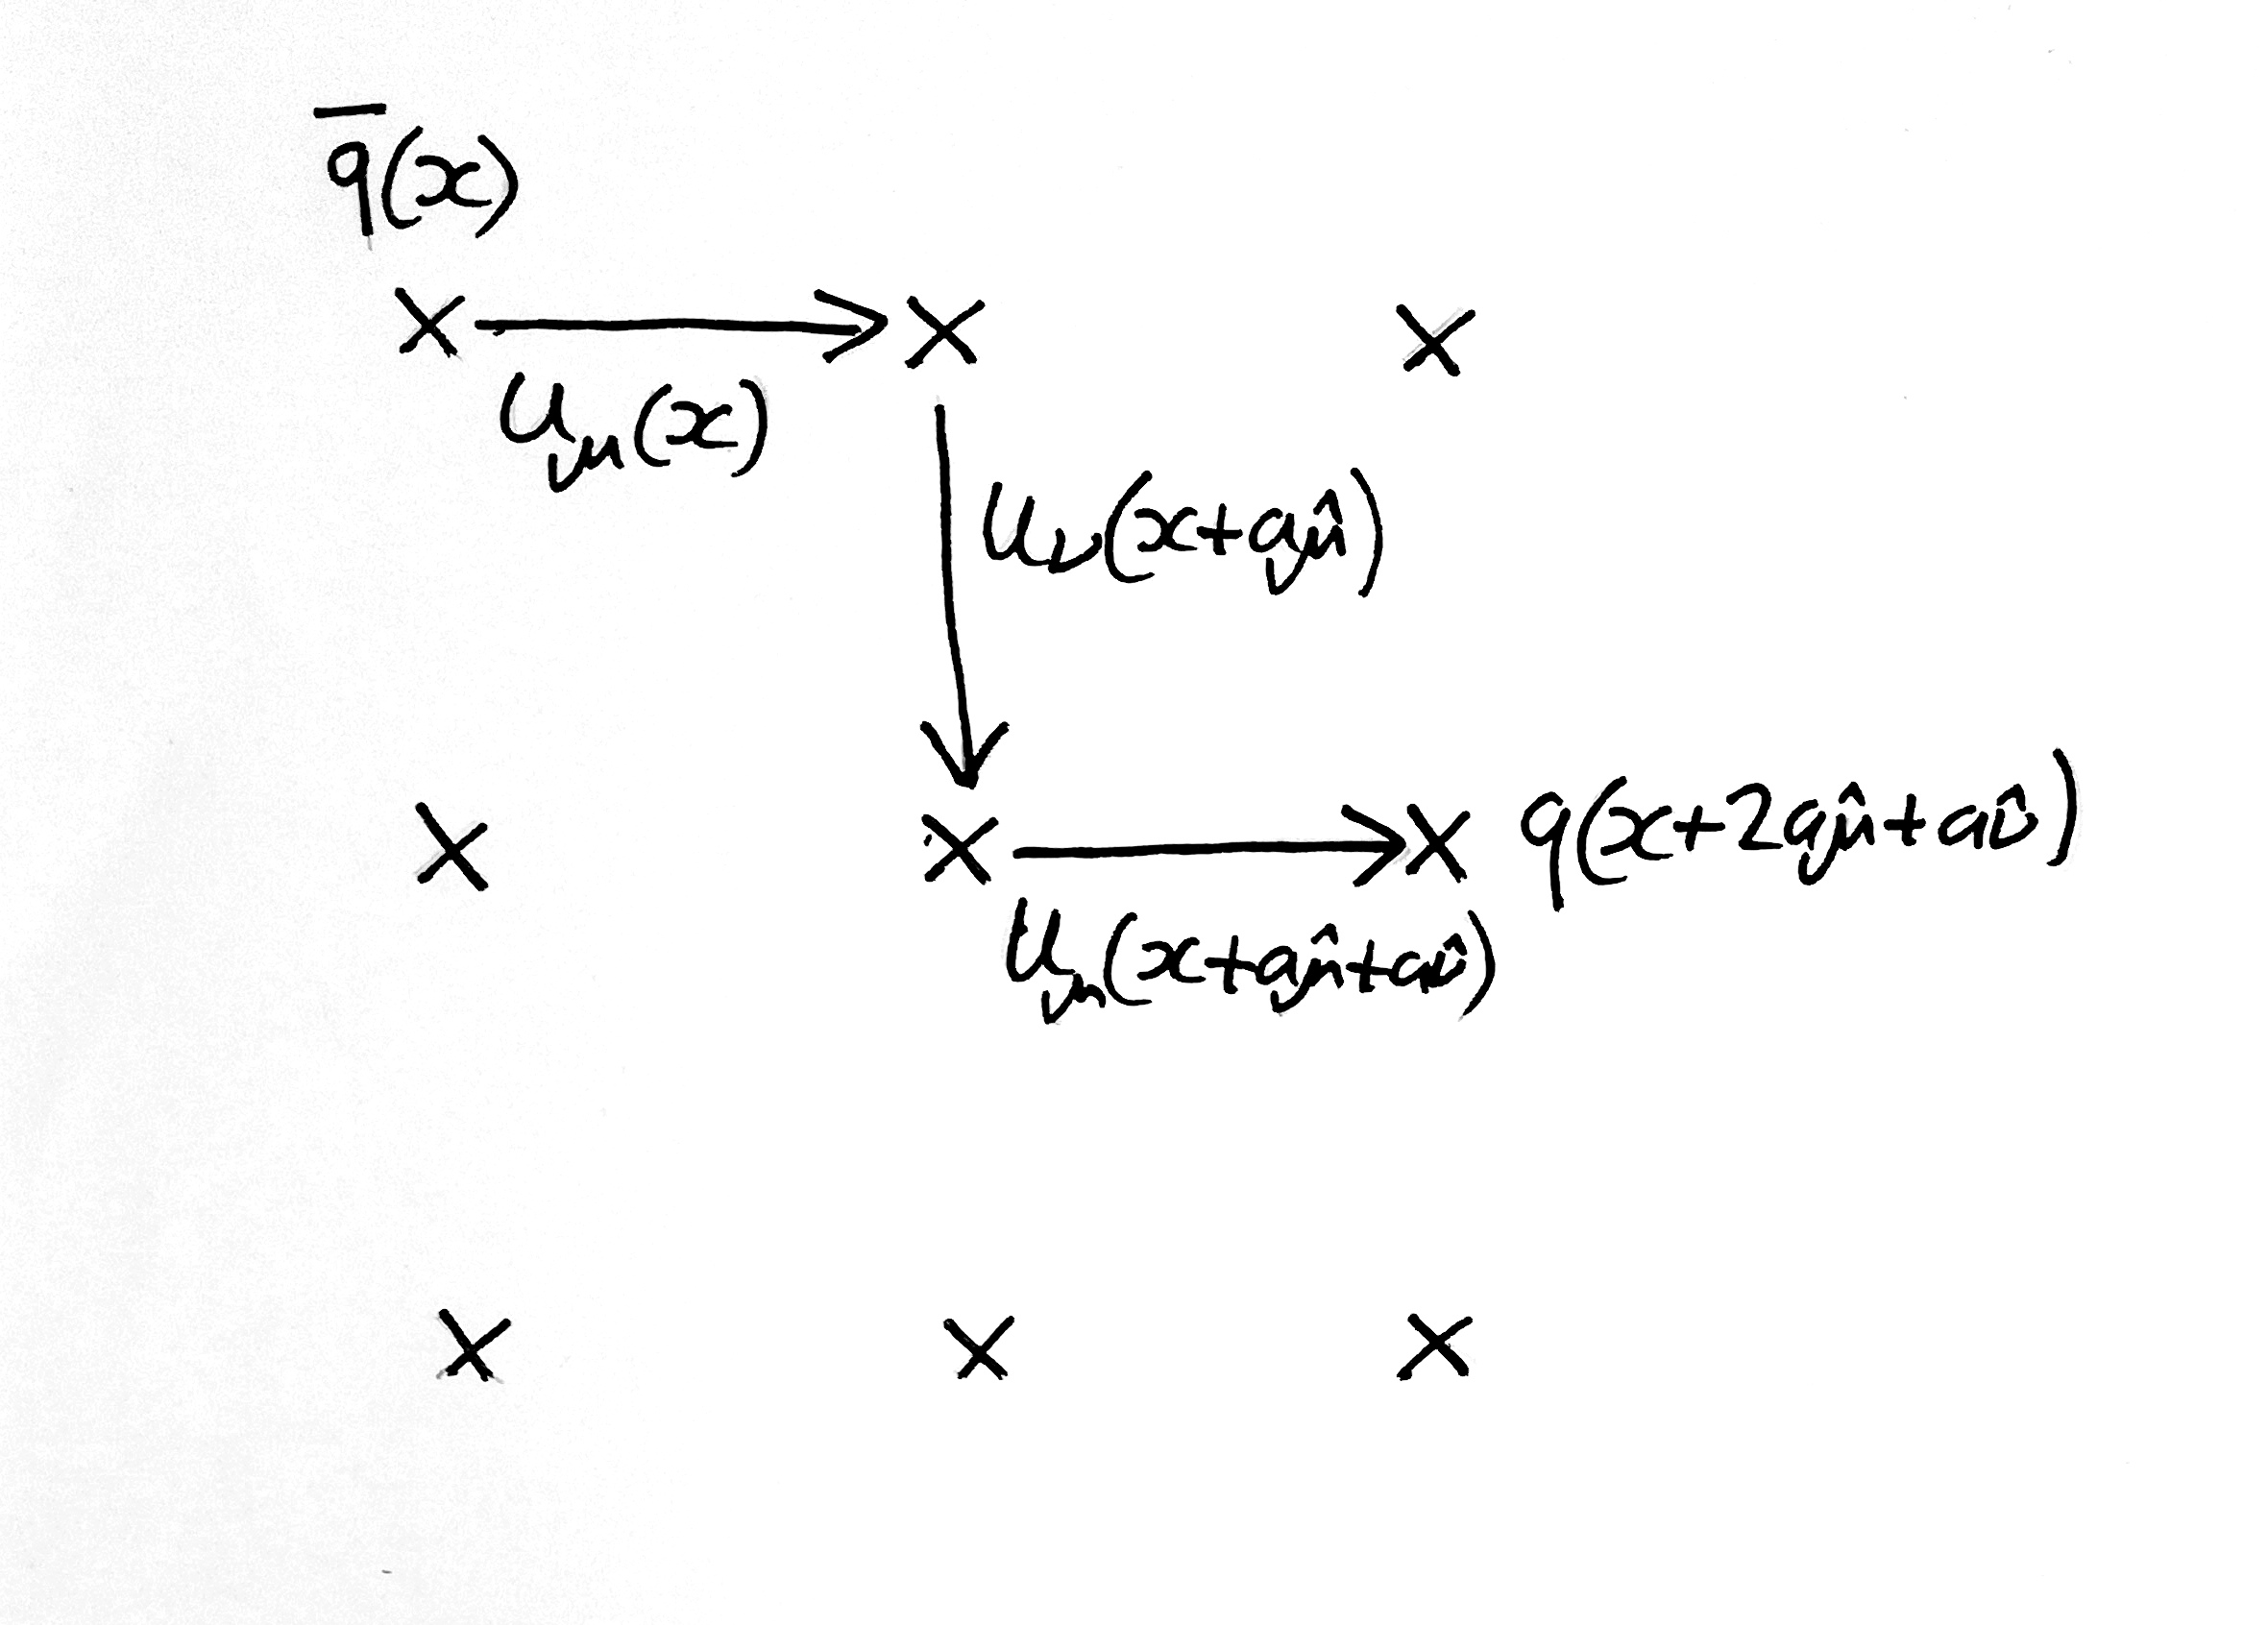
\includegraphics[width=0.55\textwidth]{images/wilson_line.jpg}
    \caption{Depiction of a gauge invariant quark bilinear, connected by a Wilson line made of gauge links.}
  \end{center}
  \vspace{-10pt}
\end{figure}

The $\bar{q}\slashed{D}q$ term in the QCD Lagrangian can then be represented on the lattice in a Gauge invariant way by
\begin{align}
  {1\over 2a}\bar{q}(x) \gamma_{\mu}(U_{\mu}(x)q(x+a\hat{\mu}) + U^{\dagger}_{\mu}(x-a\hat{\mu})q(x-a\hat{\mu}) ).
  \label{eq:latticederivative}
\end{align}
If one defines the links in terms of the the continuum gauge fields $G_{\mu}$ via
\begin{align}
  U_{\mu}(x) = \exp\left( iga G_{\mu}\left(x+{a\hat{\mu}\over2}\right) \right),
\end{align}
then \eqref{eq:latticederivative} takes the correct form in the continuum limit, i.e. it becomes $\bar{q}\slashed{D}q + \order{a^2}$.

\subsection{The Gauge Action}

We must design a pure gauge part of the action in terms of link variables. It is clear that the only gauge-invariant operator that depends only on the link variables are closed loops of links, as in fig. \ref{fig:plaquette}.

\begin{figure}[htb!]
  \begin{center}
    \vspace{-10pt}
    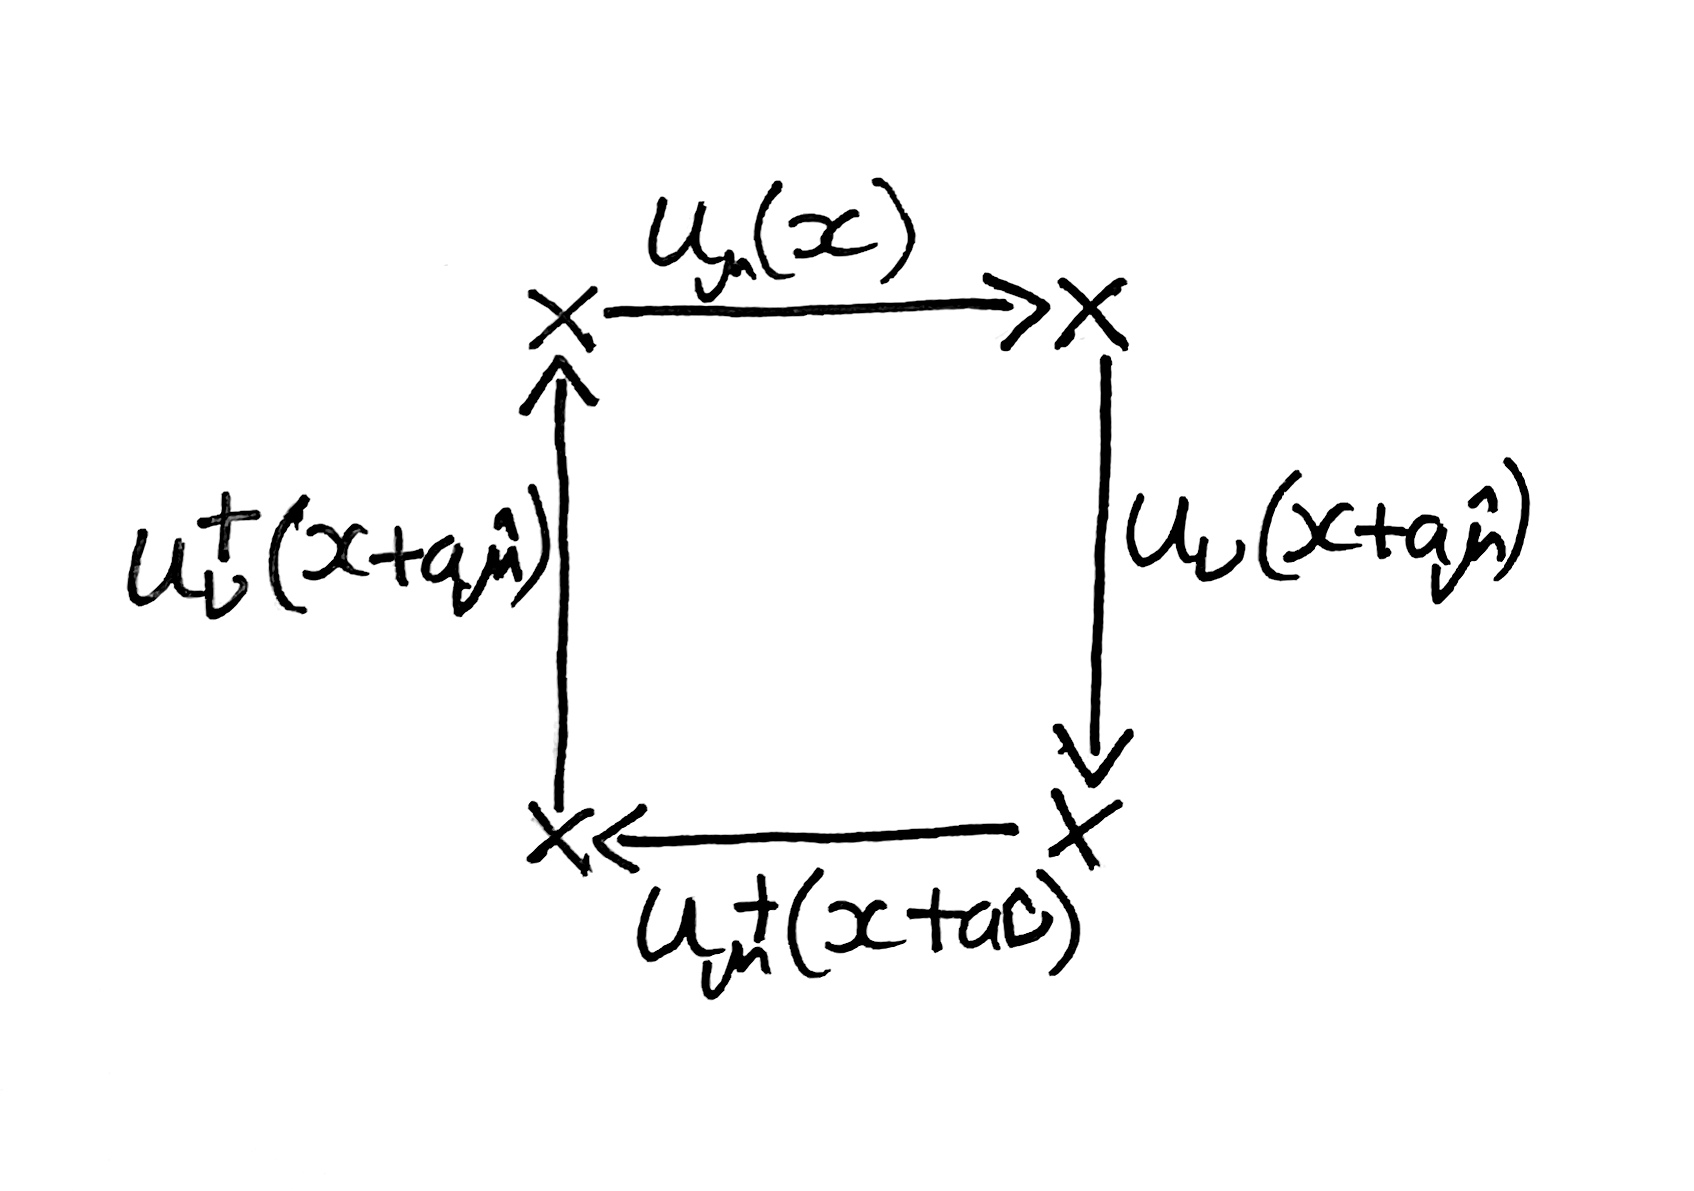
\includegraphics[width=0.55\textwidth]{images/plaquette.jpg}
    \vspace{-15pt}
    \caption{Elementary Plaquette. \label{fig:plaquette}}
  \end{center}
\end{figure}

This brings us basically all the way to a legitimate lattice gauge action. The simplest lattice discretisation of the Yang-Mills action is the real part of the smallest possible closed loop of gauge links;
\begin{align}
  S_G = - &{1\over g^2} \sum_x \sum_{\mu\neq \nu} \text{Re Tr} (1-\Box_{\mu\nu}(x)), \\
  &\Box_{\mu\nu} = U_{\mu}(x)U_{\nu}(x+a\hat{\mu}) U^{\dagger}_{\mu}(x+a\hat{\nu}) U^{\dagger}_{\nu}(x).
  \label{eq:wilson_gauge_action}
\end{align}
$\Box_{\mu\nu}$ is called the {\it{elementary plaquette}}. In the continuum limit this action reduces to
\begin{align}
  S_G = {1\over 4} \int d^4x \text{Tr}G_{\mu\nu}G^{\mu\nu} + \order{a^2},
\end{align}
as required.

%This lattice action can be understood in terms of the geometrical interpretation of gauge theory. The gauge force is due to {\it{curvature}} in the gauge field, a path-dependence in parallel transport. 

In fact, any closed loop reduces to the Yang-Mills action in the continuum. This can be seen intuitively, taking the continuum limit means shrinking any closed loop into an infinitesimally small point. We can choose a gauge action made of any combination of closed loops, so what is the optimal choice?

\subsection{Symmanzik Improvements of the Gauge Action}
\label{sec:symmanzik_gauge}

Any lattice action is admissible for a calculation as long as it reduces to the appropriate QCD action in the continuum. This gives us a lot of freedom in how we chose our lattice action. %A pure gauge action can be any combination of closed Wilson loops.

This freedom can be exploited in order to push expectation values of observables on the lattice closer to their continuum values (reduce the 'discretisation effects'). %such that if one needed to perform an extrapolation of some expectation value to the continuum, the extrapolation would be better controlled.
This program is known as {\it{Symmanzik improvement}}.

In general, a sensible lattice action can be written as
\begin{align}
  S = \sum_{i} c_i \mathcal{O}^i_{\text{lat}} = z_0(\{c_i\}) S_{\text{cont}} + a^2 \sum_{n=1} z_n(\{c_i\}) S_n\,,
  \label{eq:continuum_limit_action}
\end{align}
where $S_{\text{cont}}$ is the continuum action. We are free to choose any $\{c_i\}$ such that $z_0(\{c_i\}) = 1$. In every example we are concerned with, $\order{a}$ terms are absent, so we ignore them here (the arguments presented here carry straightforwardly to situations with $\order{a}$ corrections). A fundemental postulate of the Symmanzik approach is that improvement of one observable (removal of discretisation effects) results in improvement of all other observables. With this in mind, a reasonable approach is:
\begin{itemize}
\item
  Choose some set of lattice operators $\{\mathcal{O}^i_{\text{lat}}\}$. The number of operators required $N$ is the number of allowed irrelevant operators in the continuum theory at mass dimension matching the order of $a$ you want to remove. This is because, formally speaking, one needs $N$ tunable $c_i$ values in order to tune $N$ $z_n(\{c_i\})$ values to zero.
\item
  Inspect the continuum limit of the lattice action to find $z_0(\{c_i\})$, enforce $z_0(\{c_i\})=1$.
\item
  Choose some observable $\mathcal{O}$ that can be calculated in both the lattice and continuum theory. Use the remaining freedom in $\{c_i\}$ to remove the leading $a$ dependence in $\langle \mathcal{O}\rangle$ order by order in perturbation theory. i.e., if we write the expectation value as
  \begin{align}
    \langle \mathcal{O} \rangle = \sum_{n,m} a^{2n} g^{2m}\langle \mathcal{O}_{n,m}(\{c_i\}) \rangle,
  \end{align}
  then this amounts to demanding that $\langle \mathcal{O}_{1,m}(\{c_i\})\rangle = 0$, for as many $m$'s as possible.
\end{itemize}

Applying this to pure QCD, this procedure results in the L\"uscher-Weitz action \cite{luscher1985}. First consider the number of operators required. In continuum pure QCD, the only dimension 4 operator is Tr$G_{\mu\nu}G^{\mu\nu}$. There are no dimension 5 operators, hence there can be no $\order{a}$ contribution to the continuum limit of a lattice action. There are three independent dimension 6 operators:
\begin{gather}
  \text{Tr} J_{\mu\nu\rho} J_{\mu\nu\rho} ,\quad
  \text{Tr} J_{\mu\mu\rho} J_{\nu\nu\rho} ,\quad
  \text{Tr} J_{\mu\mu\nu} J_{\mu\mu\nu}, \\
  J_{\mu\nu\rho} = [ D_{\mu}, G_{\nu\rho} ] \nonumber
\end{gather}
Hence we require 3 extra operators in the lattice action to be tuned in order to remove the three contributions from the $a^2$ terms in Eq. \eqref{eq:continuum_limit_action}. The simplest choice is to take the plaquette action \eqref{eq:wilson_gauge_action}, and add all possible Wilson loops contanining 6 links. This set consists of three families related by hypercubic invariance, {\it{rectangles}} (a), {\it{parallelograms}} (b) and {\it{chairs}} (c), depicted in fig. \ref{fig:LuscherWeitz}.

\begin{figure}
  \begin{center}
    \vspace{-10pt}
    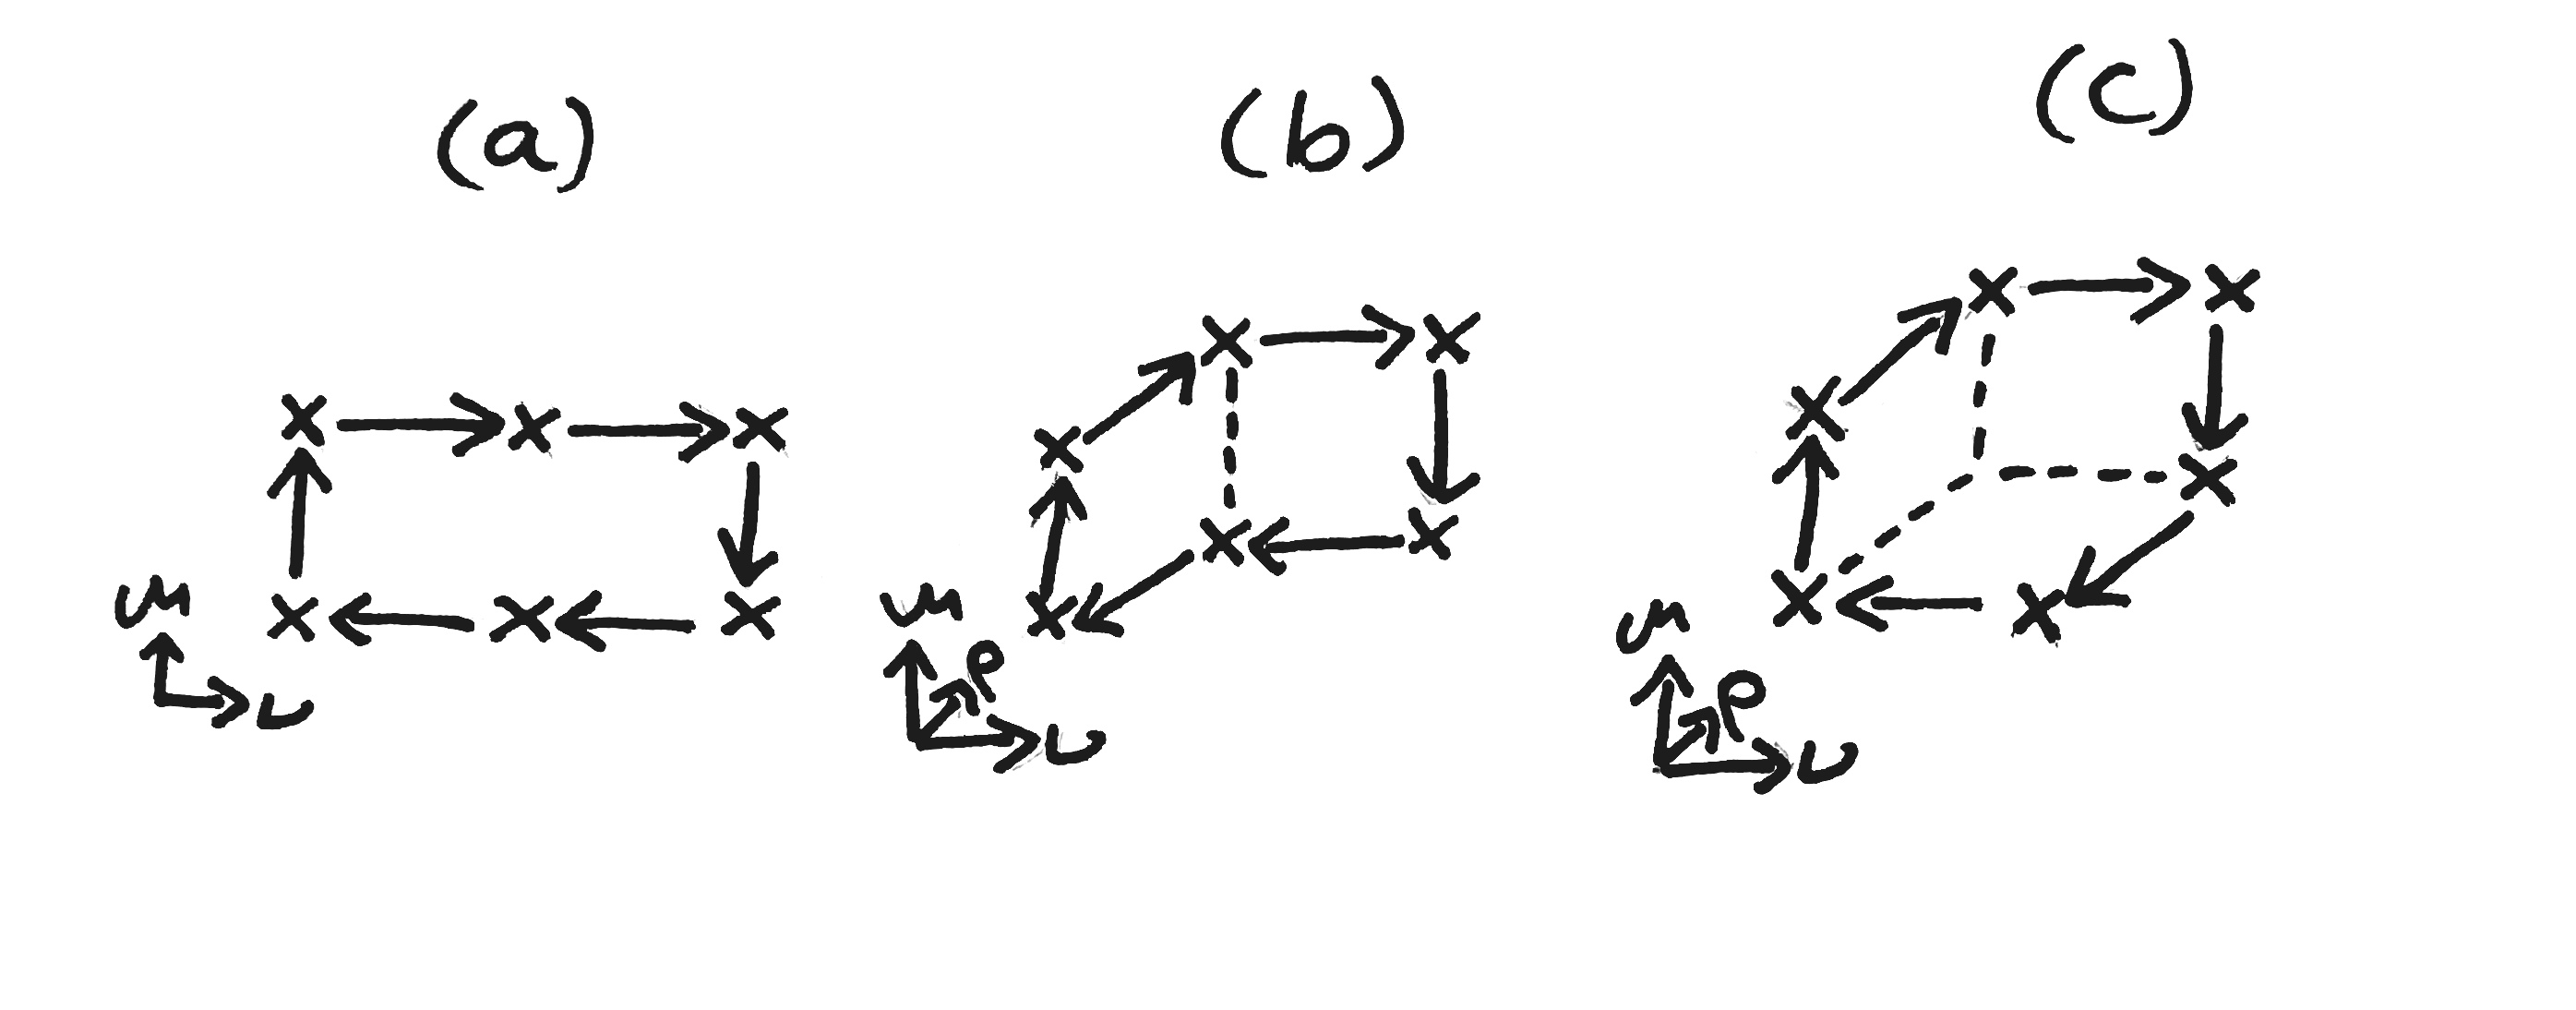
\includegraphics[width=0.85\textwidth]{images/LuscherWeitz.jpg}
    \vspace{-10pt}
    \caption{Terms additional to the elementary plaquette in the improved pure QCD action. \label{fig:LuscherWeitz}}
    \vspace{-10pt}
  \end{center}
\end{figure}

So the new lattice action is
\begin{align}
  S_G =& - {1\over g^2} \sum_x \sum_{\mu\neq \nu}(\quad c_0 \text{Re Tr} (1-\Box_{\mu\nu}(x)) + c_1 \,\text{Re Tr} (1 - \Box^a_{\mu\nu}(x)) \\
  & + \sum_{\rho\neq \mu,\nu}( \,c_2\, \text{Re Tr} (1 - \Box^b_{\mu\nu\rho}(x)) + c_3 \, \text{Re Tr} (1 - \Box^c_{\mu\nu\rho}(x))\quad)\quad)
\end{align}
where $\Box^{a,b,c}_{\mu\nu(\rho)}$ are the Wilson loops in fig. \ref{fig:LuscherWeitz}. Expanding this in small $a$, one finds the function $z_0(\{c_i\})$, setting this to one we find the condition \cite{WEISZ19831};
\begin{align}
  c_0 + 8 (c_1 + c_2) + 16 c_3 = 1.
\end{align}
The rest of the freedom must be fixed by comparing observables in the lattice and continuum theories. In \cite{WEISZ1984397} for example, by matching the gluon propagator between the two theories, one constrains the coefficients further to find
\begin{align}
  c_1 = -{1\over 12} \,,\quad\quad
  c_0 - 8c_3 = {5\over 3}.
\end{align}
These are tree-level relations, so will only prevent lattice artifacts up to $\order{\alpha_s}$. For better improvement, one must compare observables that are sensitive to loop corrections. A popular choice of observable is the so-called static quark potential $V(L)$, this is the potential energy between two static color charges, as a function of separation $L$ between them.
%% It can be related to the expectation value of a rectangular Wilson loop $\Box(L,T)$, extending in one spacial direction by $L$ links and in the time direction by $T$ links. In the $T\to \infty$ limit, this can be written as
%% \begin{align}
%%   \langle \text{Re Tr} \Box(L,T) \rangle \propto \int [d\psi d\bar{\psi} dU] e^{-\sum_x \mathcal{L} + igaA_0 \delta_{{\textbf{x}},{\textbf{x}}_0}  - igaA_0 \delta_{{\textbf{x}},{\textbf{x}}_1} }
%% \end{align}
%% where $\textbf{x}_0$, $\textbf{x}_1$ are two spacial indices $L$ links apart. This can be interpreted as the partition function $Z$ in the presence of two (oppositely charged) static color charges at $\textbf{x}_1$ and $\textbf{x}_2$. From statistical mechanics, the partition function is related to the internal energy of the system via $E = -{1\over T} \ln Z$. This motivates the expression for the static quark potential:
%% \begin{align}
%%   V(L) = - \lim_{T\to \infty} {1\over T} \ln \left( {1\over N} \langle \text{Re Tr} \Box(L,T) \rangle \right),
%% \end{align}
%% where $aN$ is the spacial extent of the lattice. To constrain $\{c_i\}$, one evaluates this order by order in perturbation theory from the continuum and lattice theories, this amounts to comparing $w_n(L,T)$ from the two theories where this is defined by
%% \begin{align}
%%   - \ln \left( {1\over N} \langle \text{Re Tr} \Box(L,T) \rangle \right) = \sum_{n=1}^{\infty} { g_0^{2n} \over (2n)! } w_n(L,T).
%% \end{align}

This procedure is affected by the presence of fermions, so it has been performed a number of times to accommodate different fermion discretisations. In this thesis we report results using the L\"uscher-Weitz action for gauge fields and Highly Improved Staggered Quarks (defined in Sec. \ref{sec:fermions}). The coefficients $\{c_i\}$ were fixed at one-loop %via $w_1(L,T)$
in \cite{Hart:2008sq} to be
\begin{align}
  c_0& = {5\over 3} + ( \,0.237088(46) - 0.1008(34) N_f \,) \alpha_s + \order{\alpha_s^2},\\
  c_1& = -{1\over 12} + ( \,-0.025218(4) + 0.0110(3) N_f \,) \alpha_s + \order{\alpha_s^2},\\
  c_2& = 0 + ( \,-0.04418(4) + 0.0016(3) N_f \,) \alpha_s + \order{\alpha_s^2}, \\
  c_3& = 0.
\end{align}
Since these have been tuned to remove $a^2$ effects up to $\alpha_s$, lattice artifacts in observables computed using this action will be of size $\order{a^2\alpha_s^2}$, so we say this action is $\order{a^2\alpha_s}$-improved.

\section{Lattice Fermions}
\label{sec:fermions}

Putting fermions on the lattice supply a much larger host of complications than gauge fields do. There exist a diverse array of approaches to dealing with fermions on the lattice adopted by different collaborations. Different actions are suited to different types of applications. The plethora of fermion actions is neccesitated by the famous {\textbf{doubling problem}}, which we will describe below.

%In this chapter we will focus only on the fermion actions used in this work; namely the Highly Improved Staggered Quark (HISQ) action, and the Non-Relativistic QCD (NRQCD) action.

Before beginning the discussion of fermion discretisations, we will define some common notation used for gamma matrices in this context. The Euclidian gamma matrices are defined to obey
\begin{align}
  \{\gamma_{\mu},\gamma_{\nu}\} = 2\delta_{\mu\nu}.
\end{align}
These have the useful property $\gamma_{\mu}^2=1$. The full set of spin-mixing matrices can be labelled according to
\begin{align}
  \gamma_n = \prod_{\mu} \left( \gamma_{\mu} \right)^{n_{\mu}}, \quad n_{\mu} = \mathbb{Z}_2.
\end{align}
We implicitly understand the product to be ordered such that $\mu=0$ is the rightmost factor and $\mu=3$ is the leftmost factor. There are 16 such matrices representing corners of the hypercube. One can also use a general site vector $x_{\mu}$ to label the matrix, then $\gamma_x = \gamma_n$ where $n_{\mu} = (x_{\mu}/a)\,\text{mod}\,2$. It is straightforward to show that for any $n$; $\gamma_n^{\dagger} \gamma_n = 1$. We also define $\gamma_{5\mu} = i\gamma_5\gamma_{\mu}$, and $\gamma_{5n} = \prod_{\mu}(\gamma_{5\mu})^n$.

\subsection{The Naive Fermion Action \& The Doubling Problem}

The interacting Dirac action is most naively discretised with
\begin{align}
  S_F &= \sum_{x,\mu} \bar{\psi}(x) \gamma_{\mu} \nabla_{\mu} \psi(x) + m\sum_x \bar{\psi}(x) \psi(x),
  \label{eq:naivefermions}
\end{align}
where $\nabla_{\mu}$ is the gauge covariant finite difference operator,
\begin{align}
  \nabla_{\mu} \psi(x) = {1\over 2a} \left( U_{\mu} (x) \psi(x+a\hat{\mu}) - U^{\dagger}_{\mu}(x-a\hat{\mu})\psi(x-a\hat{\mu}) \right).
  \label{eq:lat_derivative}
\end{align}
%% In appendix \ref{sec:doublingprob} we describe the doubling problem. This is the observation that the propagator for a fermion obeying \eqref{eq:naivefermions}, $M^{-1}(k)$ has the property
%% \begin{align}
%% M^{-1}(k+{\pi\over a}\zeta) = \gamma_{5\mu} M^{-1}(k) \gamma_{5\mu}
%% \end{align}
%% For 16 4-vectors $\zeta_{\mu} \in \mathbb{Z}_2$. This leads to 16 poles in the fermion specturm, therefore 16 distinct excitations (called \textit{tastes}). We require a way of removing the 15 unphysical excitations.
$S_F$ is invariant under a so-called {\it{doubling symmetry}}, which is generated by
\begin{align}
  \label{eq:doublingsymmetry}
  \psi(x) & \to \mathcal{B}_{\mu} \psi(x) \equiv  (-1)^{x_{\mu}/a} \gamma_{5\mu} \psi(x), \\
  \bar{\psi}(x) & \to \bar{\psi}(x)\mathcal{B}^{\dagger}_{\mu} \equiv (-1)^{x_{\mu}/a} \bar{\psi}(x) \gamma^{\dagger}_{5\mu}.
\end{align}
The product space of these form a group of 16 elements $\{\mathcal{B}_{\zeta}\}$, labeled by vectors $\zeta$ with $\zeta_{\mu}\in \mathbb{Z}_2$ (e.g. the element $\mathcal{B}_{0}\mathcal{B}_{1}$ is labeled by $\zeta=(1,1,0,0)$).

The physical significance of this symmetry can be seen when we study its effect on the action. First, notice that
\begin{align}
  \mathcal{B}_{\mu} \psi(x) & = \gamma_{5\mu} \sum_k \tilde{\psi}(k) e^{i(k+{\pi\over a}\hat{\mu})\cdot x} \\
  & = \gamma_{5\mu} \sum_k \tilde{\psi}\left(k-{\pi\over a}\hat{\mu}\right)e^{ik\cdot x},
\end{align}
where $\{k\}$ is a discrete set of 4-momenta, with $k_{\mu}=\pi/an_{\mu}, n_{\mu}\in[1,N_{\mu}]$. The action in momentum space can be written as
\begin{align}
  S = \sum_k \bar{\tilde{\psi}}(k) M(k) \tilde{\psi}(k).
\end{align}
After the operation of $\mathcal{B}_{\mu}$ it becomes
\begin{align}
  S \to \sum_k \bar{\tilde{\psi}}(k) \gamma_{5\mu} M\left(k+{\pi\over a}\hat{\mu}\right)\gamma_{5\mu} \tilde{\psi}(k).
\end{align}
Since we know $S$ is invariant under this transformation, it must be true that $\gamma_{5\mu} M\left(k+{\pi\over a}\hat{\mu}\right)\gamma_{5\mu} = M(k)$, and therefore
\begin{align}
  \boxed{  \quad M^{-1}\left(k+{\pi\over a}\hat{\mu}\right) = \gamma_{5\mu} M^{-1}(k) \gamma_{5\mu}. \quad}
  \label{eq:doubling}
\end{align}
    {\it{This}} it the doubling problem. $M^{-1}$ is the momentum space propagator for the fermion field, so Eq. \eqref{eq:doubling} shows that the spectrum of the fermion is periodic, with a period of $\pi/a$. We expect a pole in $M^{-1}(k)$ where $k \sim m$, $m$ is the pole mass of the fermion. But due to \eqref{eq:doubling} there will now be a second pole at $m + \pi/a$. %This will be around the natural cutoff imposed by the lattice $1/a$, and any higher poles like $m+2\pi/a$ is far above the cutoff so will not contribute.

    Generalizing this argument to all elements of the doubling symmetry, we see that
    \begin{align}
      M^{-1}\left(k+{\pi\over a}\zeta\right) = \gamma_{5\zeta} M^{-1}(k) \gamma_{5\zeta}.
    \end{align}
    This leads to 16 poles in the fermion specturm, one for each $\zeta$ choice, therefore 16 distinct excitations. We cal these excitations \textit{tastes}.

    One can isolate a single taste by a block-scaling procedure. Define
    \begin{align}
      \psi^{(\zeta)}(x_B) = {1\over 16} \sum_{\delta x_{\mu} \in \mathbb{Z}_2} \mathcal{B}_{\zeta}(x_B + \delta x) \psi(x_B + \delta x).
      \label{eq:block-scaling}
    \end{align}
To understand why this only contains one of the tastes, consider the $\zeta = 0$ case. This would only contain the original non-doubler taste since all other poles at $|k|\sim\pi/a$ have been integrated out. For $\zeta \neq 0$, the $\mathcal{B}_{\zeta}$ operator pushes the $\zeta$ doubler to where the $\zeta=0$ taste originally was in $k$ space, then the blocking procedure integrates out the rest.

    %% \begin{figure}
    %%   \vspace{-10pt}
    %%   \begin{center}
    %%     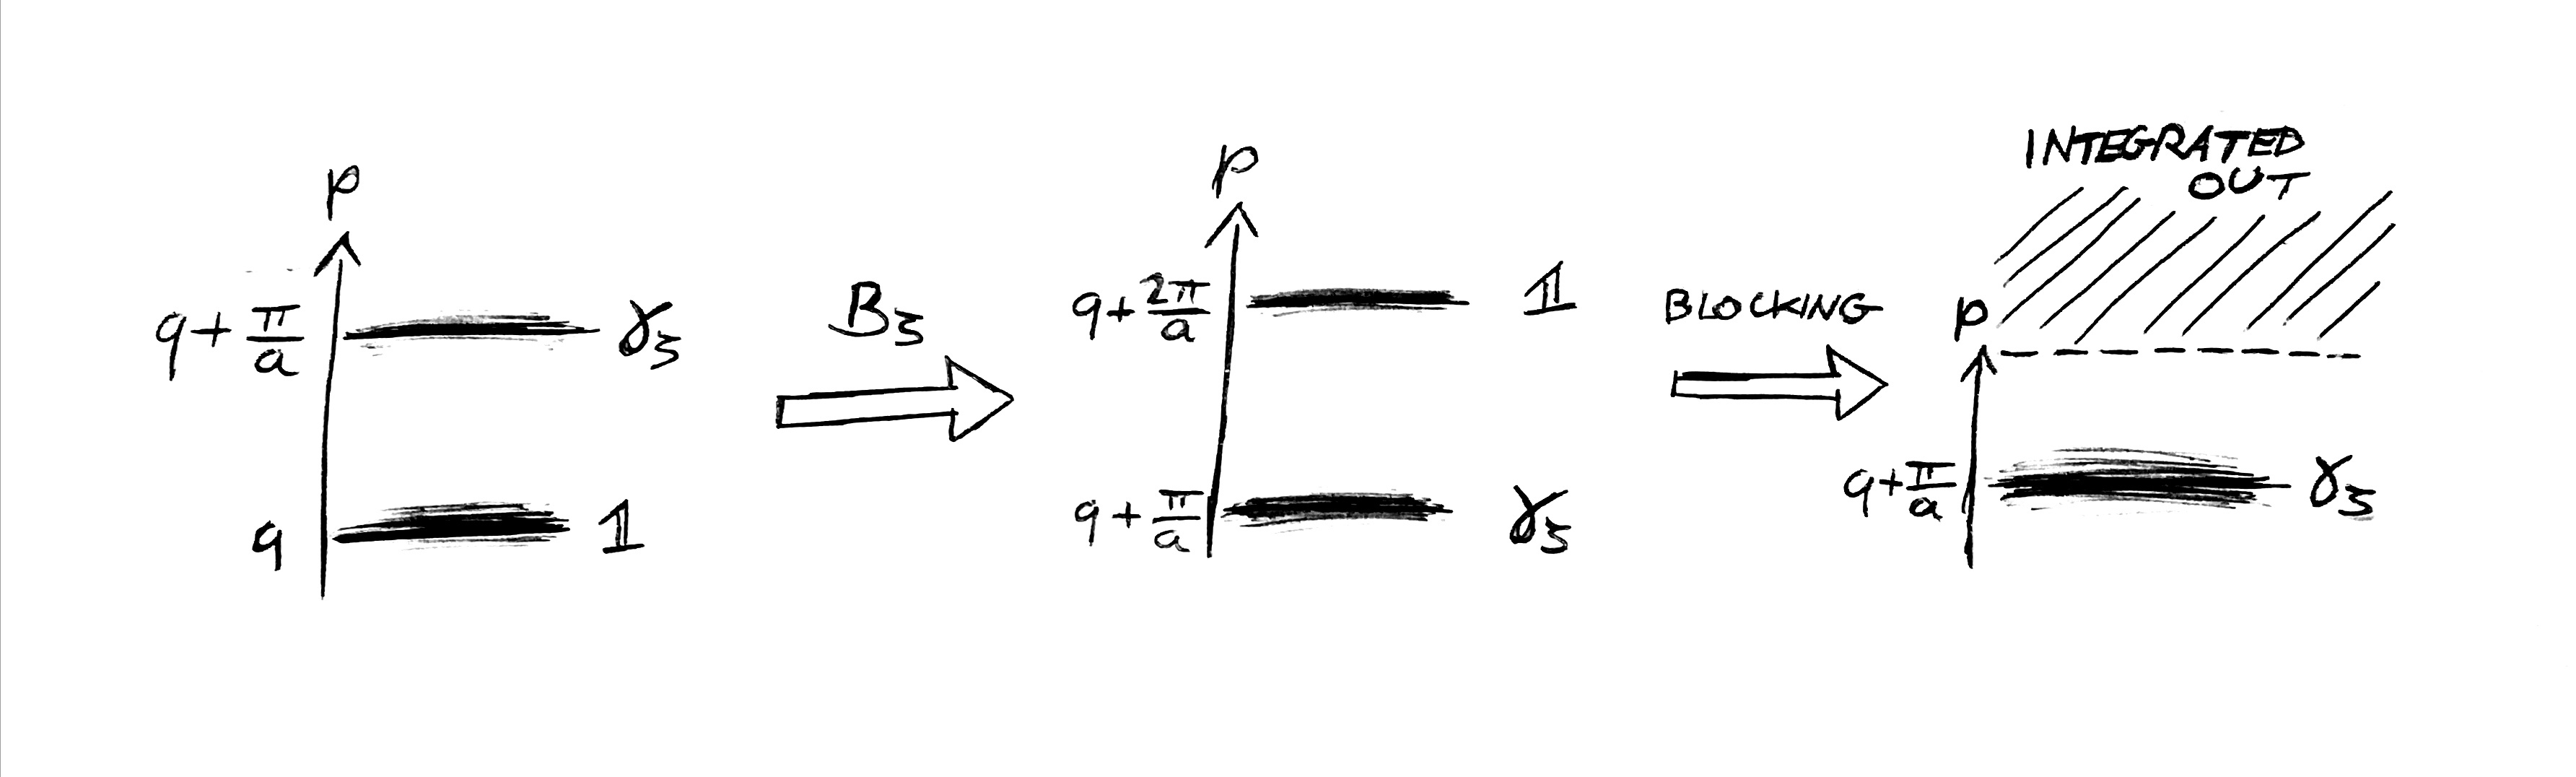
\includegraphics[width=
    %%       1.0\textwidth]{images/blocking.jpg}
    %%   \end{center}
    %%   \vspace{-25pt}
    %%   \caption{Illustration of isolating a single taste via a doubling symmetry transformation $\mathcal{B}_{\zeta}$ then a block-scaling.}
    %%   \label{fig:tastemixing}
    %% \end{figure}

    \subsection{Staggered Quarks}
    \label{sec:staggeredquarks}

    There are a number of solutions to the doubling problem. The most straightforward is to modify the action to push the mass of the unwanted tastes above the momentum cutoff, preventing it from influencing the dynamics. These are called \textit{Wilson-type fermions} \cite{Wilson:1974sk}. However, actions of this type explicitly break Chiral symmetry. Among other issues, this causes additive renormalization of the fermion mass, immensely complicating renormalization procedures.

    Another approach, known as \textit{staggered fermions} \cite{Kogut:1974ag}, partially resolves the doubling issue while retaining a remnant chiral symmetry. The work presented in this thesis makes extensive use of the staggered formalism.
    %Other notable approaches besides Wilson and staggered quarks include \textit{domain wall} \cite{Jansen:1994ym} and \textit{overlap} \cite{Narayanan:2011qj} fermions.

    Staggered fermions are defined via the following. Redefine the fields according to
    \begin{align}
      \psi(x) = \Omega(x) \chi(x),
      \label{eq:staggered}
    \end{align}
    where $\Omega(x)=\gamma_x$. In terms of the new spinor variables $\chi(x)$, the naive action \eqref{eq:naivefermions} becomes
    \begin{align}
      S_F &= \sum_{x,\mu} \bar{\chi}(x)(\alpha_{\mu}(x) \nabla_{\mu} + m ) \chi(x)
    \end{align}
    where $\alpha_{\mu}(x) = (-1)^{\sum_{\nu < \mu} x^{\mu}/a}$. The action is now diagonal in spin, leading to 4 grassman variables with identical actions and identical coupling to the gauge field. As a result, $\chi$ propagators (on fixed gauge backgrounds) are spin-diagonal:
    \begin{align}
      M^{-1}_{\chi}(x,y) = g(x,y) \,\, 1_{\text{spin}},
    \end{align}
    where $g(x,y)$ is a singlet under spin. One need only to include a single component of $\chi$ in a simulation (i.e. fix $\chi = (\chi_1,0,0,0)$), then they can compute $M^{-1}_{\chi}(x,y)[U]$ to obtain $g(x,y)$. Then, using the inverse of Eq. \eqref{eq:staggered}, $g(x,y)$ can be transformed to a propagator of the original spinors:
    \begin{align}
      M_{\psi}^{-1}(x,y) = g(x,y) \,\,\Omega(x)\Omega^{\dagger}(y).
    \end{align}
    This is clearly computationally beneficial, since one only need simulate one spinor component. But also, by only having one spinor component, one reduces the number propagating degrees of freedom by a factor of 4, cutting the number of tastes from 16 down to 4.

    I will show more explicitly how this happens. To do this, consider rewriting an isolated taste (as in Eq. \eqref{eq:block-scaling}) in the staggered formalism, i.e., in terms of $\chi$;
    \begin{align}
      \psi^{(\zeta)}(x_B) = {1\over 16} \sum_{\delta x_{\mu} \in \mathbb{Z}_2} \Omega(\delta x) \mathcal{B}_{\zeta}(0) \chi(x+\delta x).
    \label{eq:chi_blockscale}
    \end{align}
    Recall we set $\chi(x) = (\chi_1(x),0,0,0)$. The product $\Omega(\delta x)\mathcal{B}_{\zeta}(0)$ is simply a product of gamma matrices, so can only serve to ``scramble'' the elements of $\chi$. Then, in the staggered formalism, all 16 tastes $\psi^{(\zeta)}$ amount to only 4 distinguishable fermions: $(\chi_1,0,0,0)$, $(0,\chi_1,0,0)$, $(0,0,\chi_1,0)$, $(0,0,0,\chi_1)$ (with factors of (-1) and $i$).

    To obtain a useful new notation for staggered quarks, we can rewrite Eq. \eqref{eq:chi_blockscale} as
    \begin{align}
      \psi^{\alpha a}(x_B) = {1\over 8} \sum_{\eta_{\mu}\in\mathbb{Z}_2} \gamma_{\eta}^{\alpha a} \chi(x_B+a\eta).
    \end{align}
$\psi^{\alpha a}$ has spin $\alpha$ and taste $a$. Define the {\it{spin-taste}} notation for operators on $\psi^{\alpha a}$ as $(\gamma_n\otimes \gamma_m)$, where $\gamma_n$ acts on the spin component $\alpha$ and $\gamma_m$ acts on the taste component $a$. 

    One can see that the first operator in the spin-taste notation correpsonds to regular spin in the continuum by writing the free fermion action in terms of $\psi^{\alpha a}$:
    \begin{align}
      \nonumber
      S =& \sum_{x_B,\mu} \bar{\psi}(x_B) \left[ (\gamma_{\mu}\otimes 1) \nabla_{\mu} + a ( \gamma_5 \otimes \gamma^*_{\mu} \gamma_5 ) \nabla^{(2)}_{\mu} + {m\over 4}\, (1\otimes 1)  \right] \psi(x_B), \\
      \nonumber
      &\nabla_{\mu}\psi(x_B) = {1\over 4a}\left( \psi(x_B+2a) - \psi(x_B-2a) \right), \\
      &\nabla^{(2)}_{\mu}\psi(x_B) = {1\over 4a^2}\left( \psi(x_B+2a) - 2\psi(x_B) + \psi(x_B-2a) \right).
    \end{align}
If we interpret $(\gamma_{\mu}\otimes 1)$ as a gamma matrix acting on spin in the continuum, we obtain the continuum Dirac action in the $a\to 0$ limit. Including interactions with the gauge field makes the $\order{a}$ term more complicated, but the argument is unchanged.

    Hence, to reproduce some current $\bar{\psi}\gamma_n\psi$ in the continuum, one can use $\bar{\psi}(\gamma_n\otimes \gamma_m)\psi$ on the lattice, where we have the freedom to choose any $\gamma_m$. In terms of $\chi$ fields these look like
    \begin{align}
      \bar{\psi}(x_B)(\gamma_n\otimes \gamma_m) \psi(x_B) = \sum_{\eta,\eta'} \text{Tr} (\gamma_{\eta} \gamma_n \gamma_{\eta'} \gamma_m) \chi^{\dagger}(x_B+a\eta) \chi(x_B+a\eta').
    \end{align}
    The $n=m$ case results in local operators in terms of $\chi$, since the trace will vanish unless $\eta=\eta'$. To build the case with $n\neq m$, one must use 'point-split' operators, i.e. $\chi^{\dagger} (x) \chi(x+\delta x)$. Each choice of $\delta x$ corresponds to a different {\it{meson taste}}, i.e, a different combination of tastes in the two valence quarks of the meson.

    In practice in lattice calculations, the remaining 4-fold multiplicity of tastes is tackled in 3 steps:
    \begin{enumerate}
    \item
      Ensure only one meson taste is created and destroyed at the source and sink of correlation functions. 
    \item
      Minimize the interaction between tastes by a modification of the action.
    \item
      Remove contributions of extra tastes in the fermion sea by taking det$M \to \sqrt[4]{\text{det}M}$ (the context required to understand this step is eludicated in Sec. \ref{sec:MCMC}).
    \end{enumerate}
    %The third step is the main source of objection to using the staggered formalism for lattice calculations. We will briefly explain this contention in chapter \ref{chap:latticecalculations}.

    %% Step 3 can be justified by the following - in the $a\to 0$ limit, det$M$ tends to (det$M^{(0)})^4$, where $M^{(0)}$ is the Dirac operator for a single taste. Then, taking the 4th root (in principle) reduces the determinant to that of a sea containing 1 taste.

    \subsection{Highly Improved Staggered Quarks}
    \label{sec:HISQ}

    \begin{figure}
      \vspace{-10pt}
      \begin{center}
        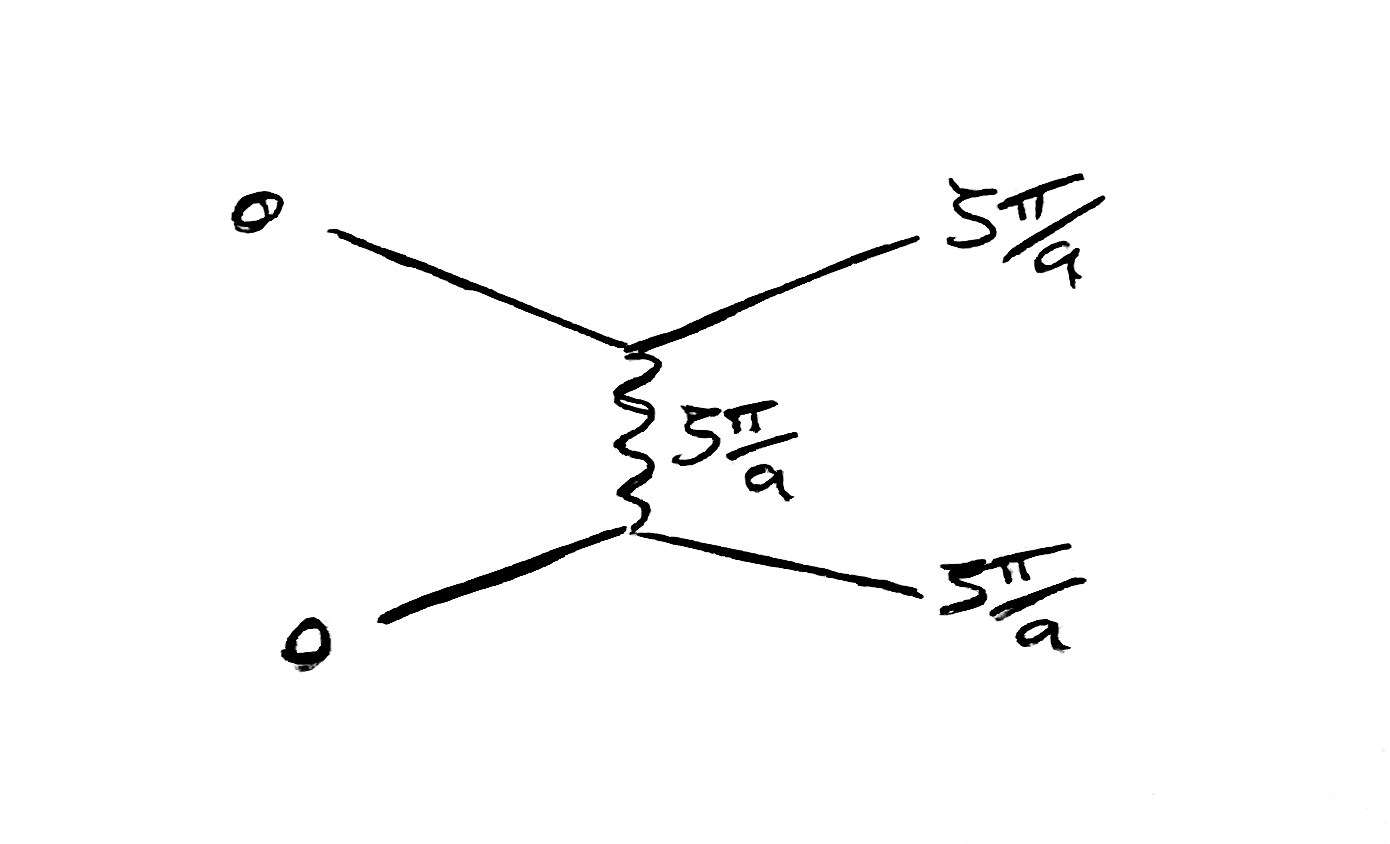
\includegraphics[width=
          0.6\textwidth]{images/taste_exchange.jpg}
      \end{center}
      \vspace{-30pt}
      \caption{Taste mixing at tree level.}
      \label{fig:tastemixing}
    \end{figure}

    Step 2 above is the guiding principle for the action we use in much of this work, the Highly Improved Staggered Quark (HISQ) action \cite{Follana:2006rc}.

    Interaction between different tastes (``taste mixing'') is dominated by the process in fig. \ref{fig:tastemixing}, the exchange of single gluons carrying momenta close to $\zeta \pi/a$. In HISQ, this is suppressed by modifying the gauge fields in such a way as to minimize the coupling between a gluon with momentum ${\zeta\pi/a}$ and the fermions, in other words, minimize the vertices in fig. \ref{fig:tastemixing}.

    To this end, one can change the action so that fermions only couple to {\textit{smeared}} gauge links, in which high-frequency excitations have been removed. Define the first and second covariant derivative operators;
    \begin{align}
      \nonumber
      \delta_{\rho}U_{\mu}(x) & \equiv {1\over a} \big( U_{\rho} (x) U_{\mu} (x + a\hat{\rho}) U_{\rho}^{\dagger}(x+a\hat{\mu}) \\
      & - U_{\rho}^{\dagger}(x-a\hat{\rho})U_{\mu}(x-a\hat{\rho})U_{\rho}(x-a\hat{\rho}+a\hat{\mu})\big),  \\
      \nonumber
      \delta_{\rho}^{(2)} U_{\mu}(x) & \equiv {1\over a^2} \big( U_{\rho}(x) U_{\mu}(x+a\hat{\rho})U^{\dagger}_{\rho}(x+a\hat{\mu}) \\
      \nonumber
      & - 2U_{\mu}(x) \\
      & + U_{\rho}^{\dagger}(x-a\hat{\rho})U_{\mu}(x-a\hat{\rho})U_{\rho}(x - a\hat{\rho} + a\hat{\mu}) \big).
    \end{align}
    With this we can define the smearing operator:
    \begin{align}
      \mathcal{F}_{\mu} = \prod_{\rho\neq\mu} \left( 1 + {a^2 \delta^{(2)}_{\rho}\over 4} \right).
    \end{align}
    HISQ uses two different smeared gauge fields defined by
    \begin{align}
      X_{\mu}(x) &\equiv \mathcal{U} \mathcal{F}_{\mu} U_{\mu}(x), \\
      W_{\mu}(x) &\equiv \left(\mathcal{F}_{\mu} - \sum_{\rho\neq\mu}{a^2(\delta_{\rho})^2\over 2} \right) \mathcal{U} \mathcal{F}_{\mu} U_{\mu}(x).
      \label{eq:gaugesmearing}
    \end{align}
    where $\mathcal{U}$ is a re-unitarization operator, that acts on a matrix $A$ like $\mathcal{U}A = A/\sqrt{A^{\dagger}A}$. The HISQ action can then be written as:
    \begin{align}
{\setlength\fboxsep{10pt} \boxed{\quad      S_{\text{HISQ}} = \sum_{x} \bar{\psi}(x) \left( \sum_{\mu} \gamma_{\mu} \left( \nabla_{\mu}(W) - {a^2\over 6}(1+\epsilon_{\text{Naik}})\nabla^3_{\mu}(X) \right) + m \right) \psi(x) \quad}}
    \end{align}
    Where $\nabla_{\mu}(Z)$ is the covariant derivative \eqref{eq:lat_derivative} with gauge links repaced with $Z$. This action in fact not only removes tree level interactions like fig. \ref{fig:tastemixing}, but also all taste mixing interactions at 1-loop.

    The $\nabla^3_{\mu}$ term is a Symmanzik improvement, it reduces the size of discretisation effects of observables computed using this action. The value of $\epsilon_{\text{Naik}}$ is fixed according to the constraint
    \begin{align}
      \lim_{\underline{p}\to 0} {E^2(\underline{p})-m^2\over \underline{p}^2} = 1.
    \end{align}
    where $E(\underline{p})$ obeys the tree-level dispersion relation from the HISQ action. Tuning $\epsilon_{\text{Naik}}$ according to this constraint gives us the expression \cite{Monahan:2012dq}
    \begin{align}
      \epsilon_{\text{Naik}} = \,&{ 4 - \sqrt{ 4 + 12 {m_{\text{tree}}\over \cosh(m_{\text{tree}}) \sinh(m_{\text{tree}})} } \over \sinh^2(m_{\text{tree}}) - 1 },
    \end{align}
    where $m_{\text{tree}}$ is the tree-level pole mass given by the expansion \cite{Follana:2006rc}
    \begin{align}
      m_{\text{tree}} &= m\Big( 1 - {3\over 80}m^4 + {23\over 2240}m^6 + {1783\over 537600 }m^8 \\ &- {76943\over 23654400} m^{10} \Big) + \order{m^{12}}. \nonumber
    \end{align}

    \section{Heavy Quarks on the Lattice}

    The large hierarchy of different quark masses in nature present a number of further complications to lattice calculations. $u$ and $d$ quarks cause huge problems due to how light they are, this will be adressed in Sec. \ref{sec:inversions}. $s$ quarks are easy.

    As quarks get heavier, we begin to encounter another problem. Discretisation effects will generally grow like the largest scale in the theory. If the observable being computed on the lattice is sensitive to the dynamics of a heavy quark of mass $m_h$, this will contain discretisation effects of size $(am_h)^n$ (where $n$ depends on how improved the action is). This is essentially due to the de Broglie wavelength of the heavy quark excitations being close to the lattice spacing, the excitations 'hide' in-between lattice sites.

    How heavy we can go is limited by two factors: the improvement of the lattice action and the lattice spacing. How fine we can get the lattice spacing is limited by computational cost. The physical size of the lattice must always be at least large enough to fit the lightest degrees of freedom in the system, namely it must be larger than the wavelength of pions. This means to get smaller lattice spacing requires increasing the number of sites on the lattice, hence increasing the computational costs (details in chapter \ref{chap:latticecalculations}).

    \begin{figure}
      \vspace{-10pt}
      \begin{center}
        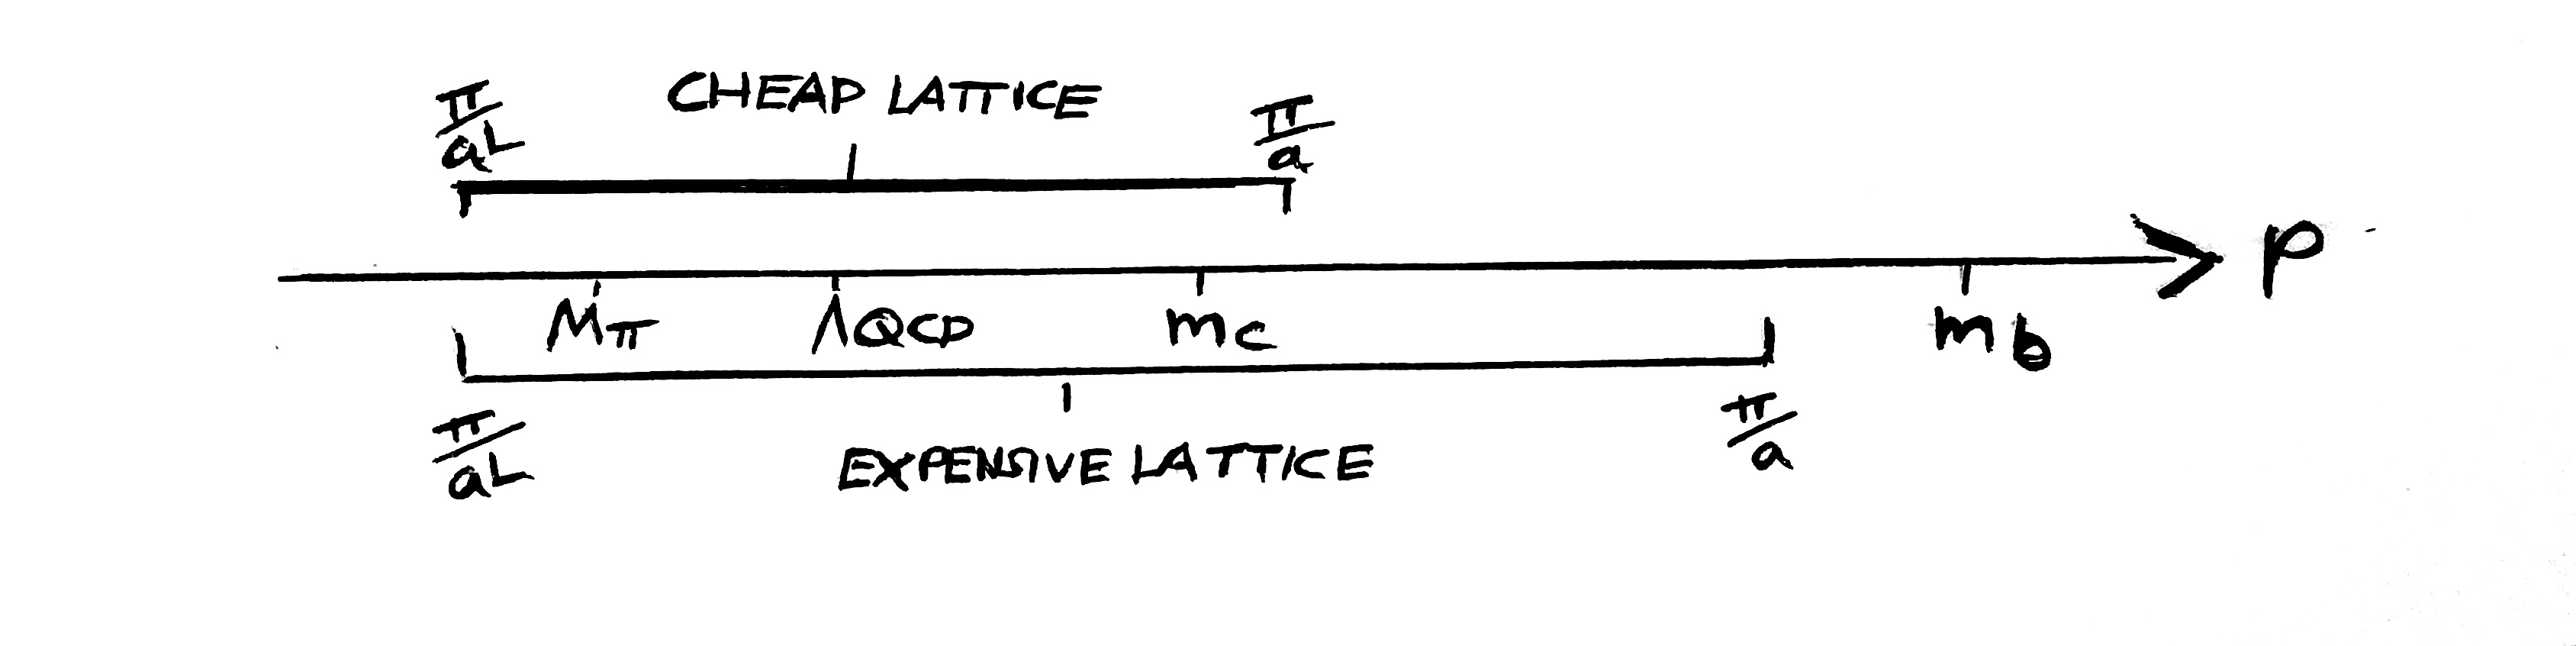
\includegraphics[width=
          0.95\textwidth]{images/scales.jpg}
      \end{center}
      \vspace{-15pt}
      \caption{Different scales relevent to non-perturbative physics, and brackets showing the range of scales that typical lattices can resolve. The larger the range of scales resolved, the more computationally expensive the calculation.}
    \end{figure}

    In the past, $c$ quarks resulted in uncontrollable discretisation effects, but now armed with highly improved actions like HISQ, and very fine lattices, $c$ physics has been conquered on the lattice \cite{Follana:2006rc,Allison:2008xk,Davies:2010ip,Donald:2012ga}.

    Physics of the $b$ quark is less well developed since the $b$ mass is so much heavier than the $c$. The $b$ can only be resolved by the very finest of lattice spacings avaliable, and using such fine lattices can be prohibitively costly. Putting physical $b$ quark on coarser lattices will create uncontrollable discretization effects.
    
    The work in this thesis concerns the decays of mesons containing $b$ quarks. We approach the issue of the heavy $b$ in two different ways, the {\it{heavy-HISQ}} approach, and the {\it{Lattice NRQCD}} approach. Since the main results of this thesis result from our heavy-HISQ studies, I will not go into too much detail in describing lattice NRQCD.

    \subsection{Heavy HISQ}

    The heavy-HISQ approach is essentially to model the $b$ with the HISQ action, but to perform the calculation at a number of unphysically light $b$ masses (that we refer to generically as heavy $h$ quarks), and extrapolate the results to the physical $b$ mass. Typically the $h$ masses span most of the region between the $c$ mass and the $b$ mass.

    Luckily there exists an effective field theory for understanding how to perform such an extrapolation - HQET. HQET gives a framework to describe how observables depend on masses of heavy quarks, so one can use HQET to derive fit forms of such an extrapolation.

    \begin{figure}
      \begin{center}
        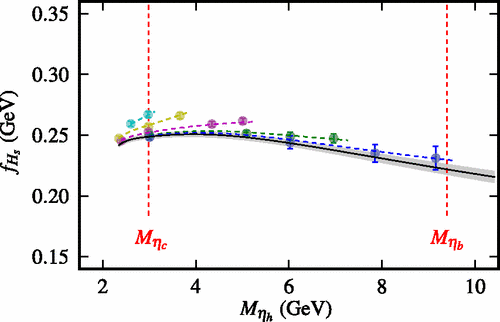
\includegraphics[width=
          0.55\textwidth]{images/fHs_heavyhisq.png}
      \end{center}
      \vspace{-5pt}
      \caption{An extrapolation to $m_h=m_b$ of the $H_s$ decay constant (where $H_s$ is a pseudoscalar $\bar{h}s$ meson)\cite{McNeile:2012qf}. The colorful points are measurements of $f_{\eta_h}$ on the lattice, the color denotes lattice spacing. The $x$ axis, $M_{\eta_h}$, is a proxy for the $h$-quark mass. \label{fig:McNeile}}
    \end{figure}

    The heavy-HISQ has so far been used for computing $b$ decay constants and masses \cite{McNeile:2011ng,McNeile:2012qf,Bazavov:2017lyh}. In \cite{McNeile:2010ji}, the approach was used to determine $c$ and $b$ quark masses and produce a new determination of $\alpha_s$. A number of heavy-HISQ calculations of semileptonic form factors are currently underway. The work presented in chapters \ref{chap:BsDsstar} and \ref{chap:BsDs} adopt the heavy-HISQ approach for computing $B_s\to D_s^*l\nu$ and $B_s\to D_sl\nu$ form factors. Besides these, there are also currently ongoing calculations of form factors for the $B_c\to \eta_cl\nu$, $B_c\to J/\psi l\nu$ \cite{Lytle:2016ixw}, $B_c\to B_sl\nu$, $B_s\to \eta_sl\nu$, and $B\to D^*l\nu$ decays.

    \subsection{Lattice NRQCD}

    The root of the problem of heavy quarks on the lattice is in the rest mass of the quark. Consider the expansion in momentum $\textbf{p}^2$ of the continuum relativistic dispersion relation:
    \begin{align}
      \omega = \sqrt{{\textbf{p}}^2 + m^2} \simeq m + {{\textbf{p}}^2\over 2m} - {{\textbf{p}}^4\over 4m^3} + ...
      \label{eq:rel_expansion}
    \end{align}
The rest mass in the first term is the source of the issue, when $m > \pi/a$ the first term pushes the frequency of excitations $\omega$ close to or  over $\pi/a$.

One could replace the relativistic fermion action e.g. HISQ, with a lattice version of NRQCD \cite{Lepage:1992tx}. In NRQCD the $b$ has no rest mass, so $b$ excitations will have frequencies much smaller than $\pi/a$.

    %% The leading order Lagrangian in the continuum is
    %% \begin{align}
    %%   \mathscr{L}^0_{NRQCD} = \psi^{\dagger}_+ \left[ i\partial_0 + {{\bf{\nabla}}^2\over 2m_b} \right] \psi_+.
    %% \end{align}
    %% $\psi_+$ is the first two components of a Dirac spinor, the second two components (the antiparticle) are not present since the dispersion relation from this Lagrangian has no antiparticle solutions.
    %% $m_b$ is the bare mass for the $b$ quark. The NRQCD action reproduces \eqref{eq:rel_expansion} with the first term chopped out.

    %% Correction terms are chosen to be all gauge-invariant terms, grouped according to powers of the quark velocity $v$. For an example of deducing such powers: kinetic enegry = $m_b v^2 = \int d^3x \psi_+^{\dagger} {\bf{\nabla}^2\over 2m_b} \psi_+$ $\rightarrow$ $|\bf{\nabla}|/m_b \sim v$.

    Another benefit of NRQCD is that it does not suffer from a doubling problem, since the doubling problem is a purely relativistic issue (the doubling symmetry requires 4 component spinors for $\gamma$ matrices to act on.

    The lattice calculations we perform require us to compute propagators for $b$ quarks on fixed gauge backgrounds. The form of the action allows propagators $G_b({\textbf{x}},t)[U]$ to be computed using a simple recursion relation
    \begin{align}
      G_b({\textbf{x}},t+1)[U] = e^{-aH}[U] G_b({\textbf{x}},t)[U],
      \label{eq:nrqcd_recursion}
    \end{align}
    which is numerically very fast in comparison to how HISQ propagators are computed (see Sec. \ref{sec:inversions}). $H$ is the NRQCD Hamiltonian. In the interest of numerical stability, the time evolution operator is re-cast as
    \begin{align}
      e^{-aH} = \left(1 - {a\delta H\over 2}\right)\left(1-{aH_0\over 2 n}\right)^n U_0^{\dagger}({\textbf{x}},t) \left(1 - {aH_0\over 2n}\right)^n \left(1-{a\delta H\over 2}\right),
    \end{align}
    where $n$ is an arbitrary integer (chosen in our studies to be $n=4$), and the Hamiltonian has been broken up into a leading part $H_0$ and correction $\delta H$. $G_b$ here are propagators for the 2-component spinor fields used in NRQCD (see Sec. \ref{sec:continuum_nrqcd}). We use the $\mathcal{O}(\alpha_s v^4)$ corrected NRQCD Hamiltionian:
    \begin{align}
      aH_0 =& - {\nabla^{(2)}\over 2am_b} , \\
      \nonumber
      a\delta H =& - c_1 {(\nabla^{(2)})^2 \over 8 (am_b)^3} + c_2{ i\over 8(am_b)^2} ( \nabla\cdot {\bf{\tilde{E}}} - {\bf{\tilde{E}}}\cdot \nabla) \\
      \nonumber
      & - c_3 {1\over 8(am_b)^2} \sigma\cdot ( \nabla\times{\bf{\tilde{E}}} - {\bf{\tilde{E}}}\times\nabla) \\
      \nonumber
      & - c_4 {1\over 2am_b} \sigma\cdot {\bf{\tilde{B}}} + c_5 {\nabla^{(4)}\over 24 am_b} \\
      & - c_6 {(\nabla^{(2)})^2\over 16n (am_b)^2},
      \label{eq:nrqcd_dH}
    \end{align}
    where $\nabla^{(2,4)}$ are the second and fourth lattice derivative, $\sigma$ are $SU(2)$ matrices acting on spin, and ${\bf{\tilde{E}}}$ and ${\bf{\tilde{B}}}$ are the (Symmanzik improved) chromoelectric and chromomagnetic fields. The form of $\nabla^{(2,4)}$,${\bf{\tilde{E}}},{\bf{\tilde{B}}}$ were defined in Sec. 4.2 of \cite{Lepage:1992tx}, and were improved upon in \cite{Gray:2005ur}.

    The coefficients $\{c_i\}$ have been fixed via various calculations adopting a number of methods. The coefficients of the kinetic terms, $c_{1,5,6}$, were most recently fixed by comparing the lattice NRQCD dispersion relation to that of the continuum in perturbation theory \cite{Davies:2018fwg}. $c_2$ is a spin-independent term which can effect radial and orbital excitation energies, this is not expected to have as large an effect as the kinetic terms, so is set to its tree-level value of 1. The result of varying $c_2$ on relevant observables was investigated in Sec. IIIC of \cite{Dowdall:2011wh}, and the effects were very small. $c_3$ and $c_4$ are spin-dependent terms, which would have a small effect on spin-averaged observables (i.e. all observables computed in this work). $c_3$ is set to 1, and $c_4$ is tuned non-perturbatively, by matching predictions of the fine structure of the $\Upsilon$ spectrum from lattice NRQCD to experiment \cite{Dowdall:2011wh}.

Another symmanzik improvement is introduced in this context by multiplying the gauge links by the so-called {\textit{tadpole factor}} $u_0 = \sum_{\mu,\nu}\langle \text{Tr}\Box_{\mu\nu} /4\rangle$. This removes the tadpole diagrams proportional to $a^2$ that appear in gluon propagators.
    
    Once the propagator for the 2-component non-relativistic $b$ quark has been found, it must be transformed back into a 4-component spinor. This is done by an inverse Fouldy-Wouthuysen transformation \cite{PhysRev.78.29}:
    \begin{align}
      \psi(x) = e^{-{{\bf{\gamma}}\cdot{\bf{\nabla}}\over 2am_b}}\binom{\psi_+(x)}{0}.
      \label{eq:FoldyWoldy}
      \end{align}
